\section{Architecture Version 1}

We are going to work on several versions of a basic architecture.  In
the future we may cluster a given virtual machine, we may add a
security layer, we may add some user interface layers, etc.  But for
now try to understand the components of this basic architecture.

\begin{figure}[h!]
  \centering
  \fbox{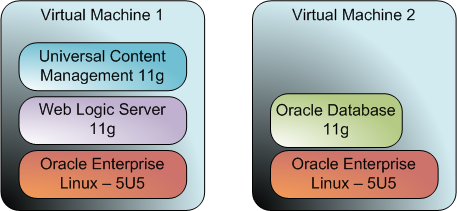
\includegraphics[width=130mm]{images/BasicArchitecture}}
  \caption{Basic Architecture}
\end{figure}

As you can see this is a two Virtual Machine system.  This can live on
either one or two physical machines.  The RAM foot print is:
	
\begin{itemize}  
\item Virtual Machine 1: (OEL5U5, WLS11g \& UCM11g) - 1.5 GigaBytes
\item Virtual Machine 2: (OEL5U5 \& ODb11g) - 1 GigaByte
\end{itemize}
	
We'll supply 10 GB disk space for each of the images.